\chapter{Embedded Sequences and Transformation Techniques}\indexmain{imperativeandstate}
\label{cha:imperativeandstate}

In this chapter we'll have a look at language constructs which allow to emit text from rules/subpatterns and which allow to execute a graph rewrite sequence at the end of a rule invocation.
The ability to execute a sequence at the end of a rule invocation allows to combine rules and build complex rules.
After a short discussion of transformation techniques we apply the language constructs introduced so far to accomplish certain common transformation tasks.

%%%%%%%%%%%%%%%%%%%%%%%%%%%%%%%%%%%%%%%%%%%%%%%%%%%%%%%%%%%%%%%%%%%%%%%%%%%%%%%%%%%%%%%%%%%%%%%%
\section{Imperative Statements}\indexmain{imperative statements}
\label{sct:imperative}

%-----------------------------------------------------------------------------------------------
\subsection{Exec and emit in rules}

The following syntax diagram gives an extensions to the syntax diagrams of the Rule Set Language chapter \ref{chaprulelang}:
\begin{rail}
  ExecStatement: 'emit' '(' StringExpr ')' ';' | 'exec' '(' RewriteSequence ')' ';'
	;
\end{rail}\ixkeyw{emit}\ixkeyw{exec}\ixnterm{ExecStatement}
The statements \texttt{emit} and \texttt{exec} enhance the declarative rewrite part by imperative clauses.
That means, i) these statements are executed in the same order as they appear within the rule,
and ii) they are executed after all the rewrite operations are done, i.e.\ they operate on the modified host graph.
However, \emph{attribute} values of deleted graph elements are still available for reading.
The \texttt{eval} statements are executed before the execution statements, i.e.\ the execution statements work on the recalculated attributes.
\begin{description}
  \item[XGRS Execution] The \texttt{exec} statement executes a graph rewrite sequence, which is a composition of graph rewrite rules. Graph elements may be yielded to def variables in the RHS pattern. See Chapter~\ref{cha:xgrs} for a description of graph rewrite sequences. The \texttt{exec} statement is one of the means available in \GrG~to build complex rules and split work into several parts, see \ref{sub:mergesplit} for a discussion of this topic.
  \item[Text Output] The \texttt{emit} statement prints a string to the currently associated output stream (default is \texttt{stdout}). See Chapter~\ref{cha:typeexpr} for a description of string expressions.
  For emitting in between the emits from subpatterns, there is an additional \texttt{emithere} statement available.
\end{description}

\begin{figure}[htbp]
\begin{example}
	The following example works on a hypothetical network flow.
	We don't define all the rules nor the graph meta model.
	It's just about the look and feel of the \texttt{exec} and \texttt{emit} statements
	\begin{grgen}
rule AddRedundancy
{
  s: SourceNode;
  t: DestinationNode;
  modify {
    emit ("Source node is " + s.name + ". Destination node is " + t.name + ".");
    exec ( (x:SourceNode) = DuplicateNode(s) & ConnectNeighbors(s, x)* );
    exec ( [DuplicateCriticalEdge] );
    exec ( MaxCapacityIncidentEdge(t)* );
    emit ("Redundancy added");
  }
}
	\end{grgen}
\end{example}
\end{figure}

\begin{example}
This is an example for returning elements yielded from an \texttt{exec} statement.
The results of the rule \texttt{bar} are written to the variables \texttt{a} and \texttt{b};
The \texttt{yield} is a prefix to an assignment showing that the target is from the outside.

	\begin{grgen}
rule foo : (A,B)
{
  modify {
    def u:A; def v:B;
    exec( (a,b)=bar ;> yield u=a ;> yield v=b) );
    return(u,v);
  }
}
	\end{grgen}
\end{example}

%-----------------------------------------------------------------------------------------------
\subsection{Deferred exec and emithere in nested and subpatterns}\label{sec:deferredexecemithere}

The following syntax diagram gives an extensions to the syntax diagrams of the Nested and Subpatterns chapter \ref{cha:nestedsub}:
\begin{rail}
  SubpatternExecEmit:
		'emithere' '(' StringExpr ')' ';' |
		'emit' '(' StringExpr ')' ';' |
		'exec' '(' RewriteSequence ')' ';'
	;
\end{rail}\ixnterm{SubpatternExecEmit}\ixkeyw{emithere}

The statements \texttt{emit}, \texttt{emithere} and \texttt{exec} enhance the declarative nested (and subpattern) rewrite part by imperative clauses.
The \texttt{emit} and \texttt{emithere} statements get executed during rewriting before the \texttt{exec} statements;
the \texttt{emithere}-statements get executed before the \texttt{emit} statements,
in the order in between the subpattern rewrite applications they are specified syntactically
(see \ref{sec:localvarorderedevalyield} for more on this).
The \texttt{exec} statements are executed i) after the rule which used the pattern they are contained in was executed and ii) in the order as they appear within the rule.
They are a slightly different version of the \texttt{exec}-statements from the \emph{ExecStatement} introduced in \ref{replclause}, only available in the rewrite parts of subpatterns or nested alternatives/iterateds
(but not in the rewrite part of rules as the original embedded sequences).
They are executed after the original rule calling them was executed,
so they can't get extended by \texttt{yield}s,
as the containing rule is not available any more when they get executed.

\begin{note}
The embedded sequences are executed after the top-level rule which contains them (in a nested pattern or in a used subpattern) was executed; they are \emph{not} executed during subpattern rewriting.
They allow you to put work you can't do while executing the rule proper (e.g. because an element was already matched and is now locked due to the isomorphy constraint) to a waiting queue which gets processed afterwards --- with access to the elements of the rule and contained parts which are available when the rule gets executed.
Or to just split the work into several parts, reusing already available functionality, see \ref{sub:mergesplit} for a discussion on this topic.
\end{note}

\begin{warning}
And again --- the embedded sequences are executed \emph{after} the rule containing them;
thus rule execution is split into two parts, a declartive of parts a) and b), and an imperative.
The declarative is split into two subparts:
First the rule including all its nested and subpatterns is matched.
Then the rule modifications are applied, including all nested and subpattern modification.

After this declarative step, containing only the changes of the rule and its nested and used subpatterns,
the deferred execs which were spawned during the main rewriting are executed in a second, imperative step;
during this, a rule called from the sequence to execute may do other nifty things,
using further own sequences, even calling itself recursively with them.
First all sequences from a called rule are executed, before the current sequences is continued or other sequences of its parent rule get executed (depth first).

Note: all changes from such dynamically nested sequences are rolled back if a transaction/a backtrack enclosing a parent rule is to be rolled back (but no pending sequences of a parent of this parent).
\end{warning}

\begin{example}
	The exec from \texttt{Subpattern sub} gets executed after the exec from \texttt{rule caller} was executed.
	\begin{grgen}
rule caller
{
  n:Node;
  sub:Subpattern();

  modify {
    sub();
    exec(r(n));
  }
}
pattern Subpattern
{
  n:Node;
  modify {
    exec(s(n));
  }
}
	\end{grgen}
\end{example}

\begin{example}
	This is an example for emithere, showing how to linearize an expression tree in infix order.
	\begin{grgen}
pattern BinaryExpression(root:Expr)
{
  root --> l:Expr; le:Expression(l);
  root --> r:Expr; re:Expression(r);
  root <-- binOp:Operator;

  modify {
    le(); // rewrites and emits the left expression
    emithere(binOp.name); // emits the operator symbol in between the left tree and the right tree
    re(); // rewrites and emits the right expression
  }
}
	\end{grgen}
\end{example}


%%%%%%%%%%%%%%%%%%%%%%%%%%%%%%%%%%%%%%%%%%%%%%%%%%%%%%%%%%%%%%%%%%%%%%%%%%%%%%%%%%%%%%%%%%%%%%%%
\section{Transformation Techniques}\label{sub:mergesplit}

In this and the following section we'll have a look at several common graph rewriting tasks and how to accomplish them in \GrG.
They could be offered directly by some dedicated operators,
but these would need so much customization to be useful in the different situations one needs them,
that we decided against dedicated operators;
instead it is on you to program the version you need yourself by combining language constructs and rules.

There are two-and-a-half means available in the \GrG-rule language to build combined, complex rules:
\begin{description}
	\item[nested and subpatterns]
which allow to match and rewrite complex patterns built in a structured way piece by piece.
With different pieces connected together, pieces to decide in between, and pieces which appear repeatedly.
	\item[embedded graph rewrite sequences]
for deferred rule execution to do work later on you can't do while executing the rule proper (e.g. because an element was already matched and is now locked due to the isomorphy constraint); or for splitting work into several parts, reusing already available functionality.
	\item[storages and storagemaps]
to store elements collected in one run and reuse them as input in another run, i.e. using multi-value variables to break up the transformation into passes. (This is the half point, as they are not a means to build a complex rule, but a means to communicate between rules building complex transformations.)
\end{description}

\noindent In the following we'll employ them to merge and split nodes, emulate node replacement grammars, copy substructures and compute flow equations over the graph structure with sets in the nodes.
Further examples can be found in \cite{CompilerOptimization} employing two storagesets switched in between for computing a wavefront running over a compiler graph and \cite{ProgramUnderstanding} using the nested and subpatterns for extracting a state machine model from a program graph.

\begin{note}
You should use the means to build complex transformations in the order given, first try to solve the problem with nested and subpatterns, if they don't get the job done (often because of the isomorphy constraint locking of already matched elements) or feel awkward then embedded graph rewrite sequences, and if these are still inadequate then storages and storagemaps; i.e. from declarative-local to imperative-global. This helps in keeping the code readable and easily adaptable. And don't forget the last resort if you must solve a task so complex that rules, control and storages are not sufficient: adding helper nodes, edges, or attributes to the graph model and the graph itself (with the visited flags being a light version of this tactic). Note: storages and storagemaps might be useful when you are experiencing performance problems, replacing a search in the graph by a lookup in a dictionary. But beware of elements already deleted from the graph still hanging out in your storage because you forgot to remove them.
\end{note}

Furthermore we'll have a look at language constructs which allow to build transformations by introducing state as a communications means between several rule applications.

Besides the normal scalar variables from the rule application control language there are set-, map-, and array-valued storages available for communicating some information between rule applications;
additionally there are several visited flags per graph element available for this means.
Both allow to split a transformation into passes mediated by their state.

\begin{note}
The storage sets are more efficient in case the count of elements of interest is a good deal smaller than the number elements in the graph; they are looked up in the set, in contrast to the visited flags, which are used by enumerating all available graph elements, filtering according to visited state.
The visited flags on the other hand are extremely memory efficient (for free as long as you use only a few of them at the same time).
\end{note}


\subsection{Merge and split nodes}\indexmain{merge node}\indexmain{split node}
Merging a node \texttt{m} into a node \texttt{n} means transferring all edges from node \texttt{m} to node \texttt{n}, then deleting node \texttt{m}.
Splitting a node \texttt{m} off from a node \texttt{n} means creating a node \texttt{m} and transferring some edges from node \texttt{n} to \texttt{m}.

In both cases there are a lot of different ways how to handle the operation exactly:
Maybe only incoming or only outgoing edges, or only edges of a certain type \texttt{T} or only edges not of type \texttt{T}; maybe the node \texttt{n} is to be retyped, maybe the edges are to be retyped.
But common is the transferring of edges; this can be handled succintly by an \texttt{iterated} statement and the \texttt{copy} operator.
In case the node opposite to an edge may be incident to several such edges, one must use an \texttt{exec} instead (or the \texttt{independent} operator \ref{rule:homspec}), as every iteration locks the matched entities, so they can't get matched twice. Not needing the opposite node one could simply leave it unmentioned in the pattern, only referencing node \texttt{n} or \texttt{m} and the edge, but unfortunately we need the opposite node so we can connect the edge copy to it.

\begin{note}
In case a simple node merging without edge retyping is sufficient the retype'n'merge clause introduced in \ref{sec:merge} offers a much simpler alternative for merging.
\end{note}

Now we'll have a look at an example for node merging: T1-T2 analysis from compiler construction is used to find out whether a control flow graph of a subroutine is reducible, i.e. all loops are natural loops. All loops being natural loops is a very useful property for many analyses and optimizations. The analysis is split into two steps, T1 removes reflexive edges, T2 merges a control flow successor into its predecessor iff there is only one predecessor available. These two steps are iterated until the entire graph is collapsed into one node which means the control flow is reducible, or execution gets stuck before, in which case the control flow graph is irreducible.
The analysis is defined on simple graphs, i.e. if two control flow edges between two basic block nodes appear because of merging they are seen as one, i.e. they are automatically fused into one. As \GrG~is built on multigraphs we have to explicitely do the edge fusion in a further step T3.

First let us have a look at T1 and T3, which are rather boring ... ehm, straight forward:

  \begin{example}
    \begin{grgen}
rule T1
{
  n:BB -:cf-> n;

  replace {
    n; // delete relexive edges
  }
}

rule T3
{
  pred:BB -first:cf-> succ:BB;
  pred    -other:cf-> succ;

  modify { // kill multiedges
    delete(other);
  }
}
    \end{grgen}
  \end{example}

The interesting part is T2, this is the first version using an iterated statement:

  \begin{example}
    \begin{grgen}
rule T2
{
  pred:BB -e:cf-> succ:BB;
  negative {
    -e->;
    -:cf-> succ; // if succ has only one predecessor
  }
  iterated {
    succ -ee:cf-> n:BB;

    modify { // then merge succ into this predecessor
      pred -:copy<ee>-> n; // copying the succ edges to pred
    }
  }

  modify { // then merge succ into this predecessor
    delete(succ);
  }
}
    \end{grgen}
  \end{example}

In case a control flow graph would be a multi-graph, with several control flow edges between two nodes, one would have to use an \texttt{exec} with an all-bracketed rule instead of the \texttt{iterated}, to be able to match a multi-\texttt{cf}-edge target of \texttt{succ} multiple times (which is prevented in the \texttt{iterated} version by the isomorphy constraint locking the target after the first match).

This is the second version using exec instead, capable of handling multi edges:

  \begin{example}
    \begin{grgen}
rule T2exec
{
  pred:BB -e:cf-> succ:BB;
  negative {
    -e->;
    -:cf-> succ; // if succ has only one predecessor
  }

  modify { // then merge succ into this predecessor
    exec([copyToPred(pred, succ)] ;> delSucc(succ));
  }
}

rule copyToPred(pred:BB, succ:BB)
{
  succ -e:cf-> n:BB;

  modify {
    pred -:copy<e>-> n;
  }
}

rule delSucc(succ:BB)
{
  modify {
    delete(succ);
  }
}
    \end{grgen}
  \end{example}

Natural loops are so advantageous that one transforms irreducible graphs (which only occur by using wild gotos) into reducible ones, instead of bothering with them in the analyses and optimizations.
An irreducible graph can be made reducible by node splitting, which amounts to code duplication (in the program behind the control flow graph).
In a stuck situation after T1-T2 analysis, a \texttt{BB} node with multiple control flow predecessors is split into as many nodes as there are control flow predecessors, every one having the same control flow successors as the original node.
(Choosing the \texttt{cf} edges and \texttt{BB} nodes which yield the smallest amount of code duplication is another problem which we happily ignore here.)

  \begin{example}
We do the splitting by keeping the indeterministically chosen first cf edge, splitting off only further cf edges, replicating their common target.

    \begin{grgen}
rule split(succ:BB)
{
  pred:BB -first:cf-> succ;
  multiple {
    otherpred:BB -other:cf-> succ;

    modify {
      otherpred -newe:cf-> newsucc:copy<succ>;
      delete(other);
      exec(copyCfSuccFromTo(succ, newsucc));
    }
  }

  modify {
  }
}

rule copyCfSuccFromTo(pred:BB, newpred:BB)
{
  iterated {
    pred -e:cf-> succ:BB;

    modify {
      newpred -:copy<e>-> succ;
    }
  }

  modify {
  }
}
    \end{grgen}
  \end{example}

The examples given can be found in the \texttt{tests/mergeSplit/} directory including the control scripts and test graphs; you may add \texttt{debug} prefixes to the \texttt{exec} or \texttt{xgrs} statements in the graph rewrite script files and call GrShell with e.g. \texttt{mergeSplit/split.grs} as argument from the \texttt{tests} directory to watch execution.


\subsection{Node Replacement Grammars}\indexmain{node replacement grammar}\indexmainsee{edNCE}{node replacement grammar}
With node replacement grammars we mean edNCE grammars \cite{NodeReplacement}, which stands for edge label directed node controlled embedding. In this context free graph grammar formalism, every rule describes how a node with a nonterminal type is replaced by a subgraph containing terminal and nonterminal nodes and terminal edges. The nodes in the instantiated graph get connected to the nodes that were adjacent to the initial nonterminal node, by connection instructions which tell which edges of what direction and what type are to be created for which original edges of what direction and what type, going to a node of what type.

This kind of grammars can be encoded in \GrG~by rules with a left hand side consisting of a node with a type denoting a nonterminal and iterateds matching the edges and opposite nodes it is connected to of interest; "of interest" amounts to the type and direction of the edges and the type of the opposite node. The right hand side deletes the original node (thus implicitely the incident edges), creates the replacement subgraph, and tells in the rewrite part of the iterateds what new edges of what directedness and type are to be created, from the newly created nodes to the nodes adjacent to the original node. (Multiple edges between two nodes are not allowed in the node replacement formalism, in case you want to handle them you've to use \texttt{exec} as shown in the merge/split example above.)

The following example directly follows this encoding:

  \begin{example}
This is an example rule replacing a nonterminal node \texttt{n:NT} by a 3-clique.
For the outgoing \texttt{E1} edges of the original node, the new node \texttt{x} receives incoming \texttt{E2} edges.
And for incoming \texttt{E2} edges of the original node, the new nodes \texttt{y} and \texttt{z} receive edges of the same type, \texttt{y} with reversed direction and \texttt{z} of the exact dynamic subtype bearing the same values as the original edges.
    \begin{grgen}
rule example
{
  n:NT;

  iterated {
    n -:E1-> m:T;

    modify {
      x <-:E2- m;
    }
  }

  iterated {
    n <-e2:E2- m:T;

    modify {
      y -:E2-> m;
      z <-:copy<e2>- m;
    }
  }

  modify {
    delete(n);
    x:T -- y:T -- z:T -- x;
  }
}
    \end{grgen}
  \end{example}

As another example for node replacement grammars we encode the two rules needed for the generation of the completely connected graphs (cliques) in two \GrG~rules. The first replaces the nonterminal node by a new nonterminal node linked to a new terminal node, connecting both new nodes to all the nodes the original nonterminal node was adjacent to. The second replaces the nonterminal node by a terminal node, connecting the new terminal node to all the nodes the original nonterminal node was adjacent to. This "we want to preserve the original edges" can be handled more succintly and efficiently by retyping which we gladly use instead of the iteration.

  \begin{example}
    \begin{grgen}
rule cliqueStep
{
  nt:NT;

  iterated {
    nt -- neighbour:T;

    modify {
      t -- neighbour;
      nnt -- neighbour;
    }
  }

  modify {
    delete(nt);
    t:T -- nnt:NT;
  }
}

rule cliqueTerminal
{
  nt:NT;

  modify {
    :T<nt>;
  }
}
    \end{grgen}
  \end{example}

The examples can be found in the \texttt{tests/nodeReplacementGrammar} directory.


\subsection{Copy structures}\label{subsub:copystructure}\indexmain{subgraph copying}\indexmainsee{copy structure}{subgraph copying}
Structures are copied in two passes, the first copying and collecting all nodes of interest, the second copying all edges of interest in between the nodes.

The first pass consists of covering the nodes of the structure one wants to copy with iterated subpatterns,
i.e. subpatterns which match from a root node on with iterateds along the incident edges into breadth,
employing a subpattern again on the node opposite to the root node to match into depth.
In the example we match the entire subgraph from a root node on, if one wants to copy a more constrained subgraph one can simple constrain the types, directions, and structures in the iterated subpattern covering the nodes.
The nodes are copied with the \texttt{copy} operators and a storagemap is filled, storing for every node copied its copy.

The second pass is started after the structure matching ended by executing the deferred execs which were issued for every node handled.
Each \texttt{exec} copies all outgoing edges (one could process all incoming edges instead) of a node:
for each edge leaving the original node towards another original node a copy is created in between the copy of the original node and the copy of the other node.
The copies are looked up with the original nodes from the storage map (which fails for target nodes outside of the subgraph of interest).
Here too one could constrain the subgraph copied by filtering certain edges.
In case of undirected edges one would have to prevent that edges get copied twice (once for every incident node). This would require a visited flag for marking the already copied edges or a storage receiving them, queried in the edge copying pattern and set/filled in the edge copying rewrite part.

  \begin{example}
The example shows very generally how a subgraph reachable from a root node by incident edges can get copied, collecting and copying the nodes along a spanning tree from the root node on, then copying the edges in between the nodes in a second run afterwards. The edges get connected to the correct node copies via a mapping from the old to the new nodes remembered in a storage-map.
    \begin{grgen}
pattern CopySubgraph(root:Node, ref oldToNew:map<Node, Node>)
{
  iterated { // match spanning tree of graph from root on
    root <--> ch:Node;
    cs:CopySubgraph(ch, oldToNew);

    modify {
      cs();
    }
  }

  modify {
    newroot:copy<root>; // copy nodes
    eval { oldToNew.add(root, newroot); }
    exec( [CopyOutgoingEdge(root, oldToNew)] ); // deferred copy edges
  }
}

rule CopyOutgoingEdge(n:Node, ref oldToNew:map<Node, Node>)
{
  n -e:Edge-> m:Node;
  hom(n,m); // reflexive edges
  nn:Node{oldToNew[n]}; nm:Node{oldToNew[m]};
  hom(nn,nm); // reflexive edges

  modify {
    nn -ee:copy<e>-> nm;
  }
}
    \end{grgen}
  \end{example}

The example can be found in the \texttt{tests/copyStructure} directory.
Without storagemaps one would have to pollute the graph model with helper edges linking the original to the copied nodes.

\subsection{Data flow analysis for computing reachability}\label{subsub:flow}\indexmain{flow equations}\indexmain{data flow analysis}\indexmain{reachability}
%todo: refine this nightly hacked section
%add dominance computation

In compiler construction, given a program graph, one wants to compute non-local properties in order to transform the program graph.
This is normally handled within the framework of data flow analysis, which employs flow equations telling how property values of a node are influenced by property values of the predecessor or successor nodes in addition to the node's local share on the overall information, with the predecessor or successor nodes being again influenced by their predecessor or successor nodes.
Property values are modeled as sets; the information is propagated around the graph until a fix point is reached (the operations must be monotone in order for a fix point to exist on the finite domain of discourse).
You might be interested in the transparencies under \url{http://www2.imm.dtu.dk/~riis/PPA/slides2.pdf} for some reading on this topic;
especially as this is a general method to compute non-local informations over graphs not limited to compiler construction.

We'll apply a backward may analysis (with only $gen$ but no $kill$ information) to compute for each node the nodes which can be reached from this node.
Reachability is an interesting property if you have to do a lot of iterated path checks:
instead of computing the itererated path with a recursive pattern each and every time you must check for it,
compute it once and just look it up from then on.
If you need to check several paths which must be disjoint you won't get around employing recursive subpatterns with one locking the elements for the other; but even in this case the precomputed information should be valuable (unless the graph is heavily connected), constraining the search to source and target nodes between which a path does exist, eliminating nodes which are not connected.

The reachability information will be stored in a storage set per node of the graph (indeed, we trade memory space for execution speed):
  \begin{example}
    \begin{grgen}
node class N
{
	reachable:set<N>;
}
    \end{grgen}
  \end{example}

The analysis begins with initializing all the storage sets with the local information about the direct successors by employing the following rule on all possible matches:
  \begin{example}
    \begin{grgen}
rule directReachability
{
  hom(n,m);
  n:N --> m:N;

  modify {
    eval { n.reachable.add(m); }
  }
}
    \end{grgen}
  \end{example}

The analysis works by keeping a global todo-set \verb#todo# containing all the nodes which need to be (re-)visited,
because the information in one of their successors changed;
this set is initialized with all nodes available using the sequence \verb#[addAllNodesToWorkset(todo)]#).

From then on in each iteration step a node \verb#n# is removed with \verb#(n)=pickAndRemove(todo)#, until the todo-set becomes empty, signaling the termination of the analysis; the node is processed by determining its successors \verb#[successors(n, succs)]#, adding the reachability information available in each successor to \verb#n# controled by the sequence\\
\verb#for{s in succs; (changed)=propagateBackwards(n,s,changed)}#.\\
If the information in \verb#n# changed due to this, the predecessors of the node are added to the workset via \verb#if{changed;[addPredecessors(n,todo)]}#.

  \begin{example}
This is the core rule of the dataflow analysis: the reachability information from the successor node \texttt{s} in its \texttt{reachable} storage attribute is added to the storage attribute of the node \texttt{n} of interest; if the storage set changes this is written to the returned variable.
    \begin{grgen}
rule propagateBackwards(n:N, s:N, var changed:boolean) : (boolean)
{
  modify {
    eval { n.reachable |= s.reachable |> changed; }
    return(changed);
  }
}
    \end{grgen}
  \end{example}

The example can be found in the \texttt{tests/dataFlowAnalysis} directory, just add \texttt{debug} before the \texttt{exec} (or \texttt{xgrs}) in \texttt{dataFlowAnalysisForReachability.grs} and watch it run.
A sample situation showing a propagation step is given in \ref{figdataflow}.
The subgraph at the top-left is already handled as you can see by the reachable set displayed in each node.

\begin{figure}[htbp]
  \centering
  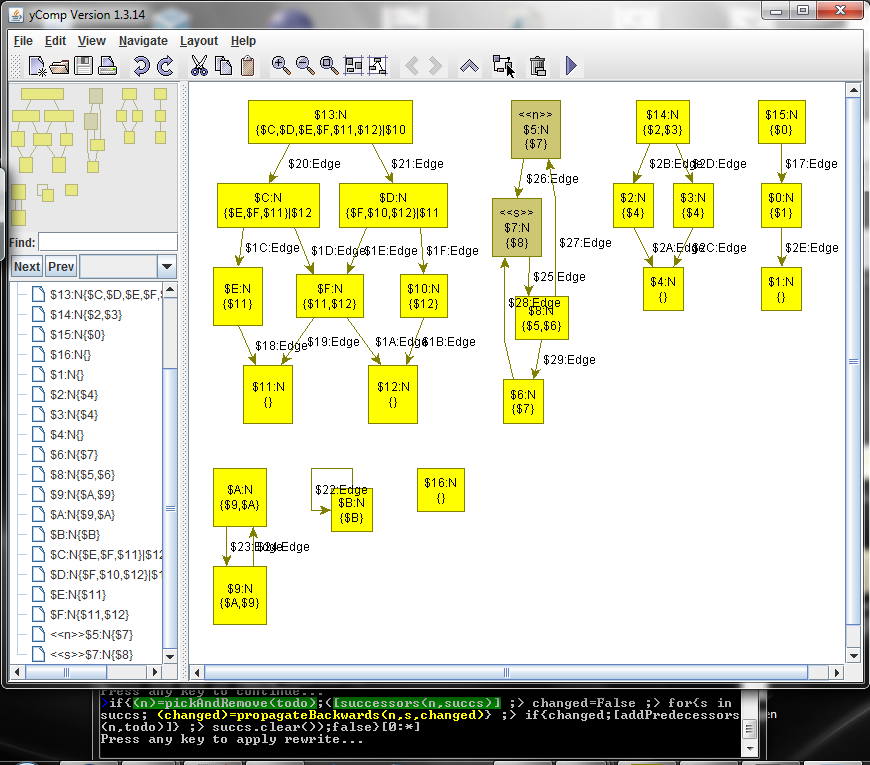
\includegraphics[width=\textwidth]{fig/Dataflow}
  \caption{Situation from dataflow analysis}
  \label{figdataflow}
\end{figure}

\subsubsection*{Worklist based data flow analysis}\indexmain{worklist}

The approach introduced above implements the basics but will not scale well to large graphs -- even medium sized graphs -- due to the random order the nodes are visited.
What is used in practice instead is a version employing a worklist built in postorder, so that a node is only visited after all its successor nodes have been processed.
For graphs without backedges, i.e. loops for program graphs, this gives an analysis which visits every node exactly once in the propagation phase.
For graphs with loops some nodes will be visited multiple times, but due to the ordering the analysis still terminates very fast.

The worklist is implemented directly in the graph by additional edges of the special type \verb#then# between the nodes, and a special node for the list start; the \verb#todo# set is kept, to allow for a fast "is the node already contained in the worklist"-check, used to save us from adding nodes again which are already contained (thus will be visited in the future anyway); i.e. the abstract worklist concept is implemented by the todo-set and the list added invasively to the graph.

  \begin{example}
    \begin{grgen}
edge class then; // for building worklist of nodes to be handled
    \end{grgen}
  \end{example}

\noindent The initial todo-set population of the simple approach is replaced by worklist constructing, successively advancing the last node of the worklist given by the \verb#last# variable; it starts with all nodes having no successor:\\
\verb#(last)=addFinalNodesToWorklist(last, todo)*#\\
Then iteratively all nodes which lead to them get added:\\
\verb#( (last)=addFurther(pos, last, todo)* ;> (pos)=switchToNextWorklistPosition(pos) )*#\\
In case of loops without terminal nodes we pick an arbitrary node from them:\\ \verb#(last)=addNotYetVisitedNodeToWorklist(last, todo)#\\
and add everything what leads to them, until every node was added to the worklist.

Now we can start the analysis, which works like the simple one does, utilizing the very same propagation rule,but follows the worklist instead of randomly picking from a todo-set, shrinking and growing the worklist along the way.

  \begin{example}
An example rule for worklist handling, adding a not yet contained node to the worklist; please note the quick check for containment via the set membership query.
    \begin{grgen}
rule addToWorklist(p:N, ref todo:set<N>, last:N) : (N)
{
  if{ !(p in todo); }

  modify {
    last -:then-> p;
    eval { todo.add(p); }
    return(p);
  }
}
    \end{grgen}
  \end{example}

  \begin{example}
An exmaple rule for worklist handling, removing the by-then processed node \texttt{pos} from the worklist.
    \begin{grgen}
rule nextWorklistPosition(pos:N, ref todo:set<N>) : (N)
{
  pos -t:then-> next:N;

  modify {
    delete(t);
    eval { todo.rem(pos); }
    return(next);
  }
}
    \end{grgen}
  \end{example}

The example can be found in the \texttt{tests/dataFlowAnalysis} directory, just add \texttt{debug} before the \texttt{exec} (or \texttt{xgrs}) in \texttt{dataFlowAnalysisForReachabilityWorklist.grs} and watch it run.
A sample situation showing a worklist building step is given in \ref{figworklist}.
The subgraph at the top-left is already handled as you can see by the reachable set displayed in each node.

\begin{figure}[htbp]
  \centering
  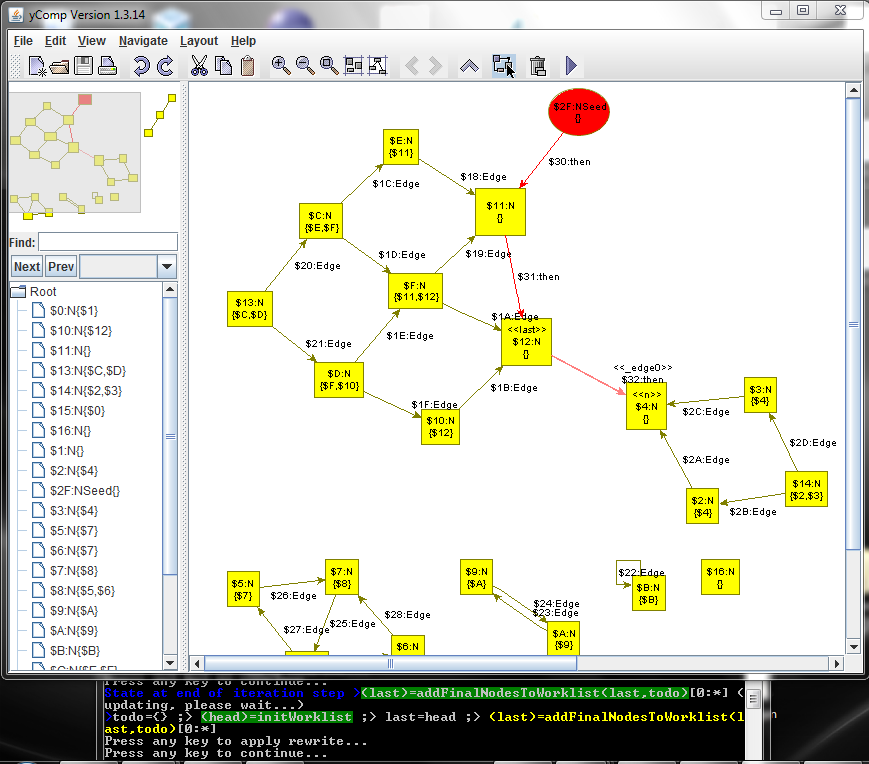
\includegraphics[width=\textwidth]{fig/Worklist}
  \caption{Situation from worklist building}
  \label{figworklist}
\end{figure}


%todo: extend, refine this quick-hacked text
\subsection{State Space Enumeration}\label{sec:statespaceenum}\indexmain{state space enumeration}

State space enumeration can be programmed in GrGen.NET utilizing the sequence constructs introduced up so far.
GrGen.NET always operates on one host graph, over one combined model, applying actions from one combined rule set --- so everything is always within reach.
That is by far the most simple approach to graph transformation, and for a tool which is not specially geared towards enumerating state spaces what makes most sense.
Thus state space enumeration (or transformation between different graphs/models) must be realized within the one host graph.
This can be achieved by virtually partitioning the host graph into smaller graphs or subgraphs, following a convention like this one:
There are nodes of type \texttt{Graph} which are representing a state of the statespace; each such representative is an  anchor node for a subgraph.
The containment in the subgraph is denoted by a \texttt{contains} edge from a node of type \texttt{Graph} to all the nodes contained in this (sub)graph.
The edges between the \texttt{Graph} nodes give the relationship between the subgraphs, i.e. successorship between the states of the statespace.
The edges between the non-\texttt{Graph} nodes are the "normal" graph edges inside the subgraphs.

The key ingredients for state space enumeration then are
\begin{itemize}
	\item The aforementioned modelling with anchor nodes linking to the subgraphs, i.e. states
	\item Backtracking angles --- they allow to recursively enumerate and apply the matches of a rule found, exhaustively stepping through the state space, rolling back the effects on the graph of the previous match tried before carrying out the next step
	\item Pause insertions --- they allow to write the interesting subgraphs found during state space search out into the host graph while effects recording of backtracking supervision is paused, so that they are not rolled back during backtracking
	\item Recursive sequences --- they allow to nest backtracking angles dynamically, so it becomes possible to enumerate an entire state space with a sequence just implementing one backtracking step
	\item The capability to create a copy of a subgraph and insert it into the host graph
	\item A subgraph attribute in the anchor nodes which contains a copy of the subgraph in the host graph, ready to be compared to the current graph, in order to decide whether that one should be inserted into the state space or purged for being an isomorphic copy of an already available instance; and of course such an equality comparison
	\item Adjacency and induced functions to compute the subgraphs from the host graph following the \texttt{contains} edges from the anchor nodes
\end{itemize}

The modelling given above allows to employ the ability of GrGen.NET/yComp to visualize nested graphs from a flat graph by interpreting node containment along edges of a special type (cf. \ref{sub:visual}), ballooning the anchor node up to a subgraph. 

An example implementation of this approach with a variant utilizing isomorphy checking and a variant without isomorphy checking can be found in the \texttt{tests/statespace} folder.
Feel free to drop in some \texttt{debug} prefixes before the \texttt{exec} (/\texttt{xgrs}) used to watch the assembling of the state space graph.

